\documentclass[12pt,a4paper]{article}
\usepackage[french]{babel}
\usepackage[utf8]{inputenc}
\usepackage[T1]{fontenc}
\usepackage{graphicx}

\title{Spécifications du Projet Planning Nouvelle Génération (PNG)}
\author{Tom BARTIER, ROBIN Yann, Marçais André, BA GUBAIR Emad}
\date{\today}

\begin{document}

\maketitle

\begin{abstract}
    Ce document décrit les spécifications des usecases "Consulter l'emploi du temps par salles" et 
    "Insérer un cours".
\end{abstract}

\section{UC "Consulter l'emploi du temps par salles"}
\subsection{}
Description : L'utilisateur connecté consulte l'emploi du temps de la salle voulue sur la semaine voulue.\\
Acteur : Utilisateur 
Déclencheur : L'utilisateur clique sur "Salle"
Pré-Condition : L'utilisateur est connecté
Post-Condition : L'emploi du temps de la salle et de la semaine choisie est affiché
\\

Scénario nominal\\
1. L'utilisateur clique sur le bouton "Salles"\\
2. Le système affiche la liste des salles\\
3. L'utilisateur clique sur le nom de la salle qui l'intéresse\\
4. Le système affiche l'emploi du temps de la salle sur une semaine\\

Scénarios alternatifs\\
Changer salle affichée\\
3. a L'utilisateur clique sur le nom de la salle\\
4. a Le système affiche toutes les salles\\
5. a L'utilisateur clique sur le nom de la salle qui l'intéresse\\
6. a Le système affiche l'EDT de la salle sur la semaine\\

Choix semaine\\
3. b L'utilisateur clique sur le numéro de la semaine qui l'intéresse\\
4. b Le système affiche l'EDT de la salle sur la semaine choisie\\


\begin{figure}[h!]
    \centering
    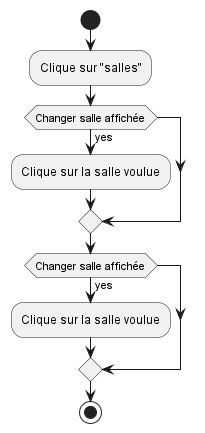
\includegraphics[width=0.8\textwidth]{Diag_activites_UC03.png}
    \caption{Description de l'image}
    \label{fig:emploi_du_temps}
\end{figure}


\section{Spécifications Fonctionnelles}
Cette section décrit les spécifications fonctionnelles du projet.

\section{Spécifications Techniques}
Cette section décrit les spécifications techniques du projet.

\section{Conclusion}
Cette section conclut le document de spécifications.

\end{document}